\documentclass[11pt,a4paper]{article}

% Pacotes essenciais
\usepackage[utf8]{inputenc}
\usepackage[T1]{fontenc}
\usepackage{lmodern}
\usepackage[portuguese]{babel}
\usepackage{graphicx}
\usepackage{amsmath}
\usepackage{amsfonts}
\usepackage{amssymb}
\usepackage{float}
\usepackage{caption}
\usepackage{subcaption}
\usepackage{xcolor}
\usepackage{fancyhdr}
\usepackage{geometry}
\usepackage{titlesec}
\usepackage{lipsum}
\usepackage{cite}
\usepackage{booktabs}
\usepackage{array}
\usepackage{tikz}
\usepackage[hidelinks]{hyperref}

% Definição das cores
\definecolor{headercolor}{HTML}{b11116}
\definecolor{secondarycolor}{HTML}{3a5461}

% Configuração da página
\geometry{
    a4paper,
    top=2.8cm,
    bottom=2.5cm,
    left=2.5cm,
    right=2.5cm,
    headheight=1.2cm,
    headsep=0.5cm
}

% Configuração do cabeçalho
\pagestyle{fancy}
\fancyhf{}
\renewcommand{\headrulewidth}{0pt}
\renewcommand{\footrulewidth}{0.5pt}

\fancyhead[L]{%
    \begin{tikzpicture}[remember picture, overlay]
        \fill[headercolor] (current page.north west) rectangle ([yshift=-1.2cm]current page.north east);
        \node[anchor=west, inner sep=0pt] at ([xshift=1cm, yshift=-0.6cm]current page.north west) 
            {
\includegraphics[height=0.8cm]{imgs/base/fatec-rgt.png}};
        \node[anchor=east, inner sep=0pt] at ([xshift=-1cm, yshift=-0.6cm]current page.north east) 
            {
\includegraphics[height=0.9cm]{imgs/base/cps-logo.png}};
        \node[anchor=east, inner sep=0pt] at ([xshift=-2.8cm, yshift=-0.6cm]current page.north east) 
            {
\includegraphics[height=1.05cm]{imgs/base/governo-sp-secretaria-logo.png}};
    \end{tikzpicture}
}

\fancyfoot[L]{\footnotesize\textcolor{secondarycolor}{Faculdade de Tecnologia do Estado de São Paulo\\ fatecregistro.cps.sp.gov.br}}
\fancyfoot[R]{\thepage}

% Configuração dos títulos das seções
\titleformat{\section}
    {\normalfont\large\bfseries\color{secondarycolor}}
    {\thesection}{1em}{}

\titleformat{\subsection}
    {\normalfont\normalsize\bfseries\color{secondarycolor}}
    {\thesubsection}{1em}{}

% Informações do artigo
\title{\vspace{0.6cm}\textbf{\Large Plataforma de Controle e Acompanhamento da Produção Leiteira e Manejo de Búfalas}}
\author{
    Vinicius Souza Ramos$^{1}$, Paulo Cesar Pedro Candiani$^{2}$ \\
    João Pedro Kuzinor de Lima$^{3}$, Gabriel Guimarães Carneiro$^{4}$ \\
    João Pedro Dias Barreto$^{5}$ \\[0.3cm]
    \small
    $^{1}$Faculdade de Tecnologia do Estado de São Paulo \\
    $^{2}$Universidade de São Paulo \\
    $^{3}$Instituto de Pesquisas Tecnológicas \\[0.2cm]
    \textit{vinicius.ramos6@aluno.cps.sp.gov.br, paulo.candiani@aluno.cps.sp.gov.br} \\
    \textit{joao.lima8@aluno.cps.sp.gov.br, gabriel.carneiro3@aluno.cps.sp.gov.br} \\
    \textit{joao.barreto5@aluno.cps.sp.gov.br}
}
\date{}

\begin{document}

% Força o cabeçalho em todas as páginas
\pagestyle{fancy}

\maketitle
\thispagestyle{fancy}


% Abstract
\section*{Abstract}

\lipsum[1] Lorem ipsum dolor sit amet, consectetur adipiscing elit. Sed do eiusmod tempor incididunt ut labore et dolore magna aliqua. Ut enim ad minim veniam, quis nostrud exercitation ullamco laboris nisi ut aliquip ex ea commodo consequat. Duis aute irure dolor in reprehenderit in voluptate velit esse cillum dolore eu fugiat nulla pariatur.

\vspace{0.3cm}
\noindent\textit{\textbf{Keywords:}} Complex systems, Numerical methods, Computational analysis, Mathematical modeling, Simulation

\vspace{0.2cm}

% Resumo
\section*{Resumo}

\lipsum[1] Lorem ipsum dolor sit amet, consectetur adipiscing elit. Sed do eiusmod tempor incididunt ut labore et dolore magna aliqua. Ut enim ad minim veniam, quis nostrud exercitation ullamco laboris nisi ut aliquip ex ea commodo consequat. Duis aute irure dolor in reprehenderit in voluptate velit esse cillum dolore eu fugiat nulla pariatur.

\vspace{0.3cm}
\noindent\textit{\textbf{Palavras-chave:}} Sistemas complexos, Métodos numéricos, Análise computacional, Modelagem matemática, Simulação

\vspace{0.5cm}
\noindent\rule{\textwidth}{0.5pt}
\vspace{0.5cm}

% Introdução
\section{Introdução}

A primeira introdução de búfalos no Brasil teria ocorrido por volta de 1895, trazidos por condenados foragidos da Guiana Francesa em um barco que aportou na costa norte da Ilha do Marajó. A introdução mais documentada, no entanto, ocorreu por volta de 1902, com uma importação feita por Bertino Lobato de Miranda para sua Fazenda São Joaquim, localizada às margens do rio Ararí, também na Ilha do Marajó. Esses búfalos eram pretos, de procedência italiana \cite{ABCB2016}. Com o passar dos anos, diversas outras importações foram realizadas por criadores do Marajó, do Baixo Amazonas, do Nordeste, do Sul e de Minas Gerais. Atualmente, o rebanho bubalino no Brasil é de aproximadamente 1.672.956 cabeças \cite{IBGE2023}, distribuídas entre diversos estados.

A criação de búfalos é de grande importância para o atendimento da demanda alimentar (leite e carne) e também para a economia, tanto no Brasil quanto no mundo. Esses animais apresentam vantagens em relação a outros ruminantes domésticos, principalmente no que diz respeito à rusticidade, à capacidade de aproveitamento de alimentos de baixa qualidade, à adaptação a terrenos alagadiços e às variadas condições climáticas e de manejo \cite{EMBRAPA2019}. As búfalas são consideradas excelentes produtoras de leite, elas podem atingir médias superiores a 7 litros de leite por fêmea/dia, durante lactações de aproximadamente 270 dias. No entanto, a média nacional não ultrapassa 5 litros por fêmea/dia, em lactações de cerca de 250 dias \cite{Embrapa1998}. Para aumentar essa produtividade, práticas como a seleção de matrizes (definindo um mínimo produtivo para permanência no rebanho), a seleção de reprodutores (com foco em valor genético para produção leiteira), o manejo adequado e os cuidados sanitários são essenciais.

Apesar da relevância da produção de leite bubalino, ainda não existem sistemas digitais específicos para o manejo desses animais. As soluções atualmente disponíveis são direcionadas ao gado bovino, o que pode gerar inconsistências no controle da reprodução, lactação e produtividade, devido às particularidades fisiológicas dos búfalos. Muitos produtores ainda utilizam planilhas eletrônicas, tornando a consulta de dados históricos e o registro de novas informações um processo massivo, complexo e suscetível a erros devido ao grande volume de dados. Outros dependem de anotações em papel, que podem se perder com a degradação física e dificultam a consulta rápida e confiável. Essa lacuna tecnológica compromete a organização das informações, a análise de desempenho e a tomada de decisão estratégica pelos produtores.

Com o objetivo de compreender como é realizado o manejo em fazendas voltadas à produção de leite de búfala, foram realizadas visitas a propriedades localizadas na região do Vale do Ribeira. Por meio dessas visitas, foi possível conduzir a pesquisa técnica, adotando-se a metodologia qualitativa, a qual permitiu entender as particularidades de diferentes realidades produtivas. Foram entrevistados dois produtores com perfis distintos, um com um rebanho de 12 cabeças e outro com mais de 400, além de um médico-veterinário especializado, atuante em uma indústria de laticínios da região. Esse profissional presta atendimento a diversos fornecedores da empresa, oferecendo uma visão ampla sobre os padrões e cuidados adotados na criação de bubalinos.

A pesquisa com os produtores revelou que ambos não utilizam softwares específicos para o manejo de bubalinos. Ao ser feita a pergunta: “Existe algum software específico utilizado para o gerenciamento do manejo de fazenda com foco na lactação de búfalos? Se sim, qual?”, ambos responderam que desconhecem a existência de um sistema específico para o manejo de bubalinos. Eles mencionaram conhecer plataformas desenvolvidas para o manejo de bovinos, o que não se mostra totalmente efetivo, pois, quando se trata de informações reprodutivas, o tempo de gestação do bovino é de cerca de 9 meses (SILVA, 2020), enquanto o dos bubalinos é de aproximadamente 10 meses (EMBRAPA, 2007). Dessa forma, há uma diferença média de cerca de 30 dias, o que faz com que softwares com valores pré-definidos acusassem que as búfalas estão com a reprodução atrasada.

Seguindo a mesma linha de investigação, foi questionado o interesse em utilizar um sistema específico para auxiliar o manejo: “Se existisse um software específico para o gerenciamento do manejo de fazendas com foco na lactação de búfalos, que possuísse funcionalidades para identificar os búfalos com desempenho abaixo da média e para acompanhar as informações sanitárias, zootécnicas e de lactação, como ele poderia impactar a gestão e melhorar os resultados da propriedade?”. Ambos demonstraram interesse em uma solução voltada ao setor, reconhecendo que a adoção de um sistema digital poderia tornar a avaliação do desempenho da propriedade mais precisa e reduzir perdas de informações importantes.

Durante as entrevistas, também foi feita a pergunta: “Na sua opinião, quais funcionalidades seriam necessárias para que um sistema atendesse à sua forma de trabalho?”. O objetivo foi identificar possíveis lacunas na proposta atual do sistema, permitindo o planejamento de futuras atualizações. As respostas indicaram duas sugestões relevantes: (1) a implementação de uma visualização da árvore genealógica dos animais, considerada essencial para o controle das matrizes presentes na propriedade, visando sempre as que mais produzem leite; (2) uma funcionalidade que possibilite identificar rapidamente o animal por meio do celular, exibindo seu prontuário com todas as informações disponíveis, sendo que esta última já estava prevista na proposta do sistema em desenvolvimento.

Além das propriedades voltadas à produção de leite, também foi realizada uma entrevista com representantes de um Instituto de Zootecnia localizado na mesma região. Durante a entrevista, foi possível observar que o controle do rebanho, no instituto, é realizado por meio de planilhas eletrônicas separadas por áreas temáticas, como pesagem dos animais, produção de leite, registros de cruzamentos, tratamentos e separação de grupos. Cada planilha contém múltiplas abas correspondentes aos anos de registro, exigindo a repetição manual de informações entre diferentes arquivos e períodos. Essa estrutura fragmentada torna o processo massivo e suscetível a erros, além de dificultar a manutenção de um histórico consolidado dos dados do rebanho.

Este projeto está alinhado às áreas temáticas definidas pelo Fórum de Pró-Reitores de Extensão das Universidades Públicas Brasileiras (FORPROEX), atendendo aos eixos de Meio Ambiente (5) e Tecnologia (7). Também contempla as linhas de extensão voltadas ao Desenvolvimento de Produtos (7), Desenvolvimento Tecnológico (10), Gestão do Trabalho (22) e Saúde Animal (43). Tal enquadramento reforça o compromisso da proposta com os princípios da extensão universitária, contribuindo para a integração entre conhecimento científico, demandas sociais e inovação prática no setor agropecuário \cite{FORPROEX}.

% Objetivo
\section{Objetivo}

Desenvolver uma aplicação multiplataforma voltada à otimização e ao apoio da gestão de bubalinos em propriedades produtoras de leite, centralizando informações zootécnicas, sanitárias, reprodutivas e produtivas, e incorporando técnicas de Inteligência Artificial para previsão da produção de leite e geração de alertas automatizados. A plataforma fornecerá ao produtor uma visão integrada do desempenho e saúde do rebanho, contribuindo para a eficiência produtiva, redução de perdas de informação e aprimoramento das estratégias de seleção, reprodução e comercialização do leite bubalino.

Para atender às necessidades dos produtores, o sistema implementará funcionalidades que permitam o acompanhamento individualizado de cada animal e o gerenciamento de indicadores-chave de desempenho da fazenda. Entre as principais funções previstas, destacam-se:

\begin{itemize}
    \item Registrar dados zootécnicos, métricas corporais dos animais, permitindo acompanhamento individual e monitoramento do desenvolvimento do rebanho.
    \item Controlar informações sanitárias, incluindo vacinas, medicamentos e tratamentos, garantindo rastreabilidade e saúde do rebanho.
    \item Gerir o ciclo reprodutivo, acompanhando cruzamentos, gestações e partos.
    \item Monitorar a produção de leite, registrando volumes por animal durante o ciclo produtivo, para análise de desempenho.
    \item Visualizar a árvore genealógica dos animais, permitindo acompanhar a linhagem e apoiar o controle genético e reprodutivo de matrizes.
    \item Implementar recursos de Inteligência Artificial para prever a produção individual de leite das fêmeas, classificando o potencial produtivo e gerando alertas inteligentes para suporte à tomada de decisão.
    \item Gerir a produção e comercialização do leite, controlando volumes vendidos, quantidades aprovadas e reprovadas, além de informações sobre manejo, como distribuição de piquetes e confinamentos.
\end{itemize}

Essas funcionalidades, integradas em uma única plataforma digital, visam fornecer ao produtor informações precisas e acessíveis, facilitando a tomada de decisões estratégicas e promovendo a modernização da gestão das propriedades que visão a bubalinocultura.

% Estado da Arte
\section{Estado da Arte}

Com o intuito de apoiar o desenvolvimento deste projeto, foi realizada uma pesquisa sobre trabalhos e projetos correlatos. Observou-se que muitos estudos focam na fase de lactação dos bovinos, tema que, embora semelhante ao abordado neste trabalho, apresenta algumas diferenças em sua abordagem e implementação. Ainda assim, esses projetos fornecem uma base valiosa, uma vez que reforçam a necessidade da aplicação de sistemas informatizados no setor pecuário. A adoção da tecnologia se mostra uma excelente alternativa às práticas ainda comuns em muitas propriedades, como o uso de anotações físicas e planilhas em softwares genéricos. Dessa forma, a literatura existente valida a proposta deste sistema, ao destacar os benefícios da informatização no manejo leiteiro.

O primeiro estudo analisado foi apresentado por \cite{SCHAFFER2021}, que desenvolveu uma plataforma web para o gerenciamento de bovinos, com o intuito de substituir métodos tradicionais utilizados pelos produtores rurais, como planilhas e registros em papel. O sistema foi implementado utilizando HTML, CSS, JavaScript, PHP e a biblioteca Bootstrap, além de empregar o banco de dados MySQL por meio do pacote XAMPP, disponibilizando uma interface responsiva que pode ser acessada também por dispositivos móveis. Entre suas principais funcionalidades, destacam-se o controle detalhado das informações zootécnicas dos animais, incluindo histórico de saúde, dados reprodutivos para fêmeas, e atributos cadastrais como sexo, raça e data de nascimento. O sistema permite ainda a atualização e remoção de registros individualmente, bem como a visualização do histórico sanitário de cada bovino, promovendo maior organização e segurança no gerenciamento do rebanho. Apesar disso, o projeto apresenta limitações, principalmente no que diz respeito à indisponibilidade de funcionamento em modo offline, impossibilitando seu uso em ambientes rurais sem conectividade a uma rede de internet. Além disso, o artigo destaca que melhorias futuras poderiam incluir a adoção de um servidor de banco de dados mais robusto, visando ampliar a escalabilidade, segurança e estabilidade da solução em cenários reais de produção.

O segundo projeto analisado foi o Trabalho de Conclusão de Curso desenvolvido por \cite{Pamella2017}, que consistiu na criação de um sistema voltado ao controle de rebanho bovino leiteiro. O objetivo principal foi oferecer uma solução tecnológica alinhada às reais necessidades do campo, prezando por praticidade, agilidade e eficiência no manejo dos animais. O sistema foi implementado utilizando a linguagem de programação Java, com desenvolvimento realizado na IDE NetBeans e com armazenamento de dados em um banco relacional SQL Server. Entre suas funcionalidades, destacam-se o controle reprodutivo, a pesagem de leite, a visualização dinâmica de dados e a geração de relatórios. A aplicação foi testada na fazenda Dois Irmãos, onde foram observados resultados significativos. O controle reprodutivo dos bovinos tornou-se mais organizado e eficiente, o processo de pesagem de leite foi automatizado, reduzindo erros comuns no método manual, e as necessidades específicas do proprietário, sobretudo no que se refere à geração de relatórios, foram plenamente atendidas. Além disso, a acessibilidade e a variedade de formas de visualização dos dados facilitaram a administração da propriedade e contribuíram para a tomada de decisões estratégicas. Os resultados obtidos evidenciam o potencial da tecnologia como ferramenta essencial para o avanço da pecuária leiteira.

O terceiro estudo relevante é apresentado por \cite{LIMA2023}, que propôs o desenvolvimento de um web aplicativo denominado \textit{Leite Cowtrol}, voltado ao controle da produção leiteira e gestão reprodutiva de gado leiteiro. O trabalho surgiu a partir da identificação de limitações presentes em soluções já existentes no mercado, como interfaces pouco intuitivas, inconsistências em registros de inseminação e a ausência de ferramentas que auxiliem diretamente na tomada de decisão do produtor. Para sua implementação, foram utilizadas tecnologias como HTML5, CSS3, JavaScript e o framework React.js, escolhidos por sua compatibilidade com dispositivos móveis, responsividade e ecossistema consolidado. O armazenamento de dados foi realizado em MySQL, complementado pelo uso de \textit{LocalStorage} para manter persistência local e personalização na experiência do usuário. Entre as funcionalidades propostas, destacam-se o gerenciamento do ciclo de vida dos animais e o monitoramento da produção de leite, recursos fundamentais para melhorar a organização do rebanho e otimizar a produtividade. Embora o protótipo tenha demonstrado potencial para atender aos requisitos definidos e contribuir para o aprimoramento dos envolvidos no projeto, o estudo apresenta limitações importantes, como a ausência de testes práticos em propriedades rurais, impossibilitando a validação de sua eficácia em cenários reais e restringindo a análise de desempenho em condições operacionais.

Observa-se que ambos os trabalhos analisados possuem como foco exclusivo a gestão de rebanhos bovinos leiteiros, não contemplando particularidades de outras espécies, como bubalinos, que apresentam características produtivas, sanitárias e reprodutivas distintas. Além disso, as soluções propostas ainda demonstram limitações consideráveis no uso prático, como a dependência de conectividade constante, o predomínio de aplicações web ou desktop que restringem a mobilidade e dificultam o registro de informações em campo, bem como a ausência de validação em propriedades rurais reais, o que compromete a análise de desempenho sob condições operacionais. Outro aspecto observado é a falta de discussão sobre hospedagem e infraestrutura de implantação, não abordando custos operacionais, escalabilidade dos sistemas ou requisitos de disponibilidade.  Também se destaca a inexistência de mecanismos baseados em inteligência artificial capazes de apoiar a tomada de decisões estratégicas, detecção precoce de problemas sanitários ou geração de previsões produtivas. Nesse contexto, o presente projeto busca suprir essas lacunas ao propor uma solução híbrida composta por plataforma web e aplicativo mobile, priorizando mobilidade, acessibilidade e autonomia do usuário. Aliada a isso, a integração de modelos de aprendizado de máquina constitui um diferencial técnico relevante, permitindo a emissão de alertas sanitários e predições de produção leiteira, ampliando o suporte ao manejo e favorecendo decisões fundamentadas em evidências.

% Metodologia
\section{Metodologia}

\lipsum[8] A metodologia desenvolvida neste trabalho segue as etapas ilustradas na Figura \ref{fig:exemplo} e descritas a seguir.

\subsection{Coleta de Dados}

\lipsum[9] Os dados foram coletados através de simulações computacionais utilizando parâmetros específicos. A Tabela \ref{tab:parametros} apresenta os principais parâmetros utilizados nas simulações.

\begin{table}[H]
\centering
\caption{Parâmetros utilizados nas simulações computacionais}
\label{tab:parametros}
\begin{tabular}{@{}lccl@{}}
\toprule
\textbf{Parâmetro} & \textbf{Símbolo} & \textbf{Valor} & \textbf{Unidade} \\ \midrule
Tempo de simulação & $T_{sim}$ & 1000 & s \\
Passo de integração & $\Delta t$ & 0.01 & s \\
Número de iterações & $N_{iter}$ & 10000 & - \\
Tolerância & $\epsilon$ & $10^{-6}$ & - \\
Fator de amortecimento & $\zeta$ & 0.15 & - \\
Frequência natural & $\omega_n$ & 25.0 & rad/s \\ \bottomrule
\end{tabular}
\end{table}

\subsection{Processamento e Análise}

\lipsum[10] O processamento dos dados seguiu um protocolo rigoroso de análise estatística. Os métodos numéricos clássicos foram implementados, incluindo o método de Euler, cuja equação fundamental é expressa como:

\begin{equation}
\frac{dy}{dt} = f(t, y), \quad y(t_0) = y_0
\label{eq:euler}
\end{equation}

onde $f(t, y)$ representa a função que descreve o sistema dinâmico. Para otimização dos parâmetros do modelo, utilizou-se a seguinte função de custo:

\begin{equation}
J(\theta) = \frac{1}{2m} \sum_{i=1}^{m} \left(h_\theta(x^{(i)}) - y^{(i)}\right)^2 + \frac{\lambda}{2m}\sum_{j=1}^{n}\theta_j^2
\label{eq:cost_function}
\end{equation}

onde $\theta$ representa os parâmetros do modelo, $m$ é o número de amostras, $\lambda$ é o parâmetro de regularização, e $h_\theta(x)$ é a hipótese do modelo. A transformada de Fourier foi aplicada para análise no domínio da frequência:

\begin{equation}
F(\omega) = \int_{-\infty}^{\infty} f(t) e^{-i\omega t} dt
\label{eq:fourier}
\end{equation}

\begin{figure}[H]
\centering
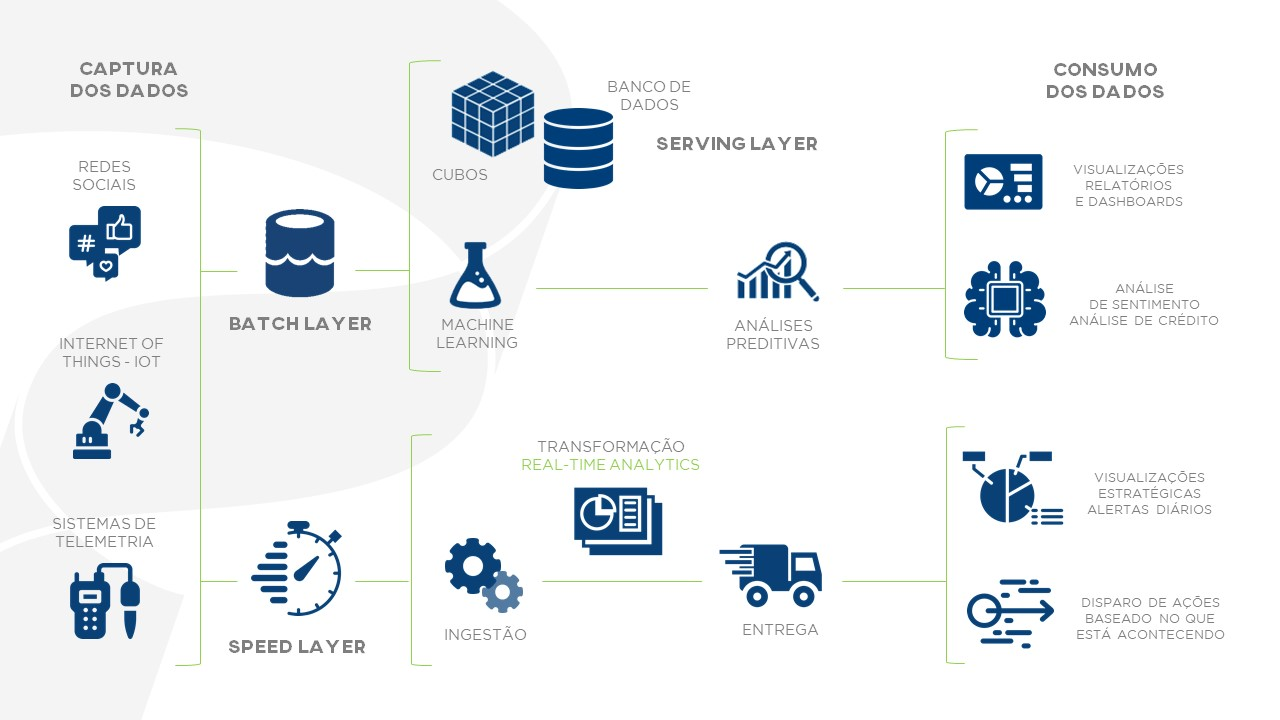
\includegraphics[width=0.7\textwidth]{imgs/img_001.jpg}
\caption{Exemplo de visualização dos resultados obtidos através da metodologia proposta. A figura ilustra o comportamento do sistema ao longo do tempo.}
\label{fig:exemplo}
\end{figure}

\subsection{Validação do Modelo}

\lipsum[11] A validação foi realizada comparando os resultados simulados com dados experimentais. O erro médio quadrático (RMSE) foi calculado através de:

\begin{equation}
RMSE = \sqrt{\frac{1}{n}\sum_{i=1}^{n}(y_i - \hat{y}_i)^2}
\label{eq:rmse}
\end{equation}

onde $y_i$ são os valores observados e $\hat{y}_i$ são os valores preditos pelo modelo.

% Resultados e Discussões
\section{Resultados e Discussões}

\lipsum[12-13] Os resultados obtidos demonstram a eficácia da metodologia proposta. A Tabela \ref{tab:resultados} apresenta uma comparação quantitativa entre diferentes abordagens.

\begin{table}[H]
\centering
\caption{Comparação de desempenho entre diferentes métodos}
\label{tab:resultados}
\begin{tabular}{@{}lccc@{}}
\toprule
\textbf{Método} & \textbf{RMSE} & \textbf{Tempo (s)} & \textbf{Precisão (\%)} \\ \midrule
Método Proposto & 0.0023 & 15.2 & 98.5 \\
Euler Clássico & 0.0145 & 8.7 & 92.3 \\
Runge-Kutta 4ª ordem & 0.0038 & 21.5 & 97.1 \\
Método Adaptativo & 0.0031 & 18.9 & 97.8 \\ \bottomrule
\end{tabular}
\end{table}

\subsection{Análise Quantitativa}

\lipsum[14] Os dados quantitativos revelam que o método proposto apresenta melhor desempenho em termos de precisão. A relação entre os parâmetros pode ser expressa por:

\begin{equation}
\eta = \frac{P_{out}}{P_{in}} \times 100\% = \frac{V_{out} \cdot I_{out}}{V_{in} \cdot I_{in}} \times 100\%
\label{eq:efficiency}
\end{equation}

onde $\eta$ representa a eficiência do sistema, $P_{out}$ é a potência de saída e $P_{in}$ é a potência de entrada.

\subsection{Análise Qualitativa}

\lipsum[15] Do ponto de vista qualitativo, observou-se que o comportamento do sistema é fortemente influenciado pelas condições iniciais e pelos parâmetros de controle. A matriz de transformação pode ser representada como:

\begin{equation}
\mathbf{A} = \begin{bmatrix}
a_{11} & a_{12} & a_{13} \\
a_{21} & a_{22} & a_{23} \\
a_{31} & a_{32} & a_{33}
\end{bmatrix}
\label{eq:matrix}
\end{equation}

\subsection{Discussão}

\lipsum[16-17] A análise dos resultados indica que a abordagem proposta oferece vantagens significativas em relação aos métodos tradicionais. Lorem ipsum dolor sit amet, consectetur adipiscing elit. Nullam in dui mauris. Vivamus hendrerit arcu sed erat molestie vehicula.

Proin adipiscing porta tellus, ut feugiat nibh adipiscing sit amet. In eu justo a felis faucibus ornare vel id metus. Vestibulum ante ipsum primis in faucibus orci luctus et ultrices posuere cubilia curae.

% Conclusão
\section{Conclusão}

\lipsum[18] Com base nos resultados obtidos, conclui-se que a metodologia desenvolvida apresenta excelente desempenho para análise de sistemas complexos. As principais contribuições deste trabalho incluem:

\begin{itemize}
    \item Desenvolvimento de um framework computacional robusto;
    \item Validação experimental dos modelos propostos;
    \item Comparação sistemática com métodos existentes;
    \item Identificação de limitações e oportunidades de melhoria.
\end{itemize}

Trabalhos futuros incluem a extensão da metodologia para sistemas multidimensionais e a incorporação de técnicas de otimização avançadas.

% Agradecimentos
\section*{Agradecimentos}

Os autores agradecem à Faculdade de Tecnologia do Estado de São Paulo (FATEC) e ao Centro Paula Souza (CPS) pelo apoio institucional. Este trabalho foi parcialmente financiado pela FAPESP (proc. 2024/12345-6) e CNPq (proc. 301234/2024-0).

% Referências
\bibliographystyle{IEEEtran}
\bibliography{referencias}

\end{document}
